Our work is based on several foundations, which we will discuss in the sections below.

\subsection{Microservice Architecture}
\label{sec:Foundation:MicroserviceArchitecture}
In a microservice architecture, the software is partitioned into many small components (``microservices''), which operate independently of each other and communicate via messages \cite{Dragoni2017}.
This software architecture style allows the construction of highly reusable components which focus on a single task (e.g. applying a watermark to a video).
This loose coupling allows for independent teams to work on different components or even the use of off-the-shelf components.
Also, scaling the application can be achieved by simply duplicating the bottlenecked microservices \cite{Dragoni2017}.
A microservice is defined by its provided- and required-interfaces, which allow for the message-exchange with other components \cite{Singh2021}.

\subsection{Asynchronous Communication}
\label{sec:Foundation:AsyncCommunication}
In the context of microservice software systems, there are two commonly used methods of communicating asynchronously.

\subsubsection{Asynchronous RESTful Communication}
\label{sec:Foundation:AsyncCommunication:REST}
\begin{figure}
\centering
  \begin{tikzpicture}[node distance=4cm,auto,>=stealth']
    \node[] (server) {MS 2};
    \node[left = of server] (client) {MS 1};
    \node[below of=server, node distance=6cm] (server_ground) {};
    \node[below of=client, node distance=6cm] (client_ground) {};
    %
    \draw (client) -- (client_ground);
    \draw (server) -- (server_ground);
    
    \draw[->] ($(client)!0.15!(client_ground)$) -- node[above,scale=1,midway]{HTTP POST Request} ($(server)!0.15!(server_ground)$);
    \draw[<-] ($(client)!0.2!(client_ground)$) -- node[below,scale=1,midway]{HTTP 202 (Accepted)} ($(server)!0.2!(server_ground)$);
    
    
    \draw[->] ($(client)!0.5!(client_ground)$) -- node[above,scale=1,midway]{HTTP GET /results} ($(server)!0.5!(server_ground)$);
    \draw[<-] ($(client)!0.55!(client_ground)$) -- node[below,scale=1,midway]{HTTP 200 (OK) with status} ($(server)!0.55!(server_ground)$);
    
    
    \draw[->] ($(client)!0.85!(client_ground)$) -- node[above,scale=1,midway]{HTTP GET /results} ($(server)!0.85!(server_ground)$);
    \draw[<-] ($(client)!0.9!(client_ground)$) -- node[below,scale=1,midway]{HTTP 303 (See Other)} ($(server)!0.9!(server_ground)$);
\end{tikzpicture}
\caption{\textbf{Asynchronous Communication using HTTP REST.} \\
MS 1 send an HTTP POST request, including the payload to MS 2. MS 2 stores the payload and starts processing. It immediately returns an HTTP Code 202 (Accepted), including a location where MS 1 can query the results (e.g. /results). Periodically, MS 1 queries the results using an HTTP GET request at the given location. If the results are not ready yet, MS 2 returns an HTTP Code 200 (OK) with the current status of the operation, otherwise it returns an HTTP Code 303 (See Other) with the location of the results.}
\label{fig:ImageAsyncHTTP}
\end{figure}

Microservices that communicate asynchronously are typically realized in one of two kinds.
Either using a RESTful pattern or using message-based communication. \\

Some systems use microservices that communicate asynchronously via asynchronous HTTP REST interfaces.
There are two interaction scenarios for this kind of asynchronous communication.
One possibility is that the initial HTTP request returns an HTTP code 202 (Accepted) and provides a location where the microservice can query the status of the operation.
When the sender queries the provided location before the operation has finished, the receiver returns the current status and information about the running operation.
Once the operation on the server has finished, the provided location will return an HTTP Code 303 (See Other) to redirect the sender to the results. \cite{Mayer2018}
This interaction is depicted in \autoref{fig:ImageAsyncHTTP}.

Alternatively, the microservice may be required to provide a callback method (e.g. a web hook, \cite{Webhooks}) where the server can send the results once the operation has finished \cite{Mayer2018}. \\

We will refer to both of these communication methods as RESTful asynchronous communication in the following paper.


\subsubsection{Message-based Communication}
\label{sec:Foundation:AsyncCommunication:MBC}

\begin{figure}
\centering
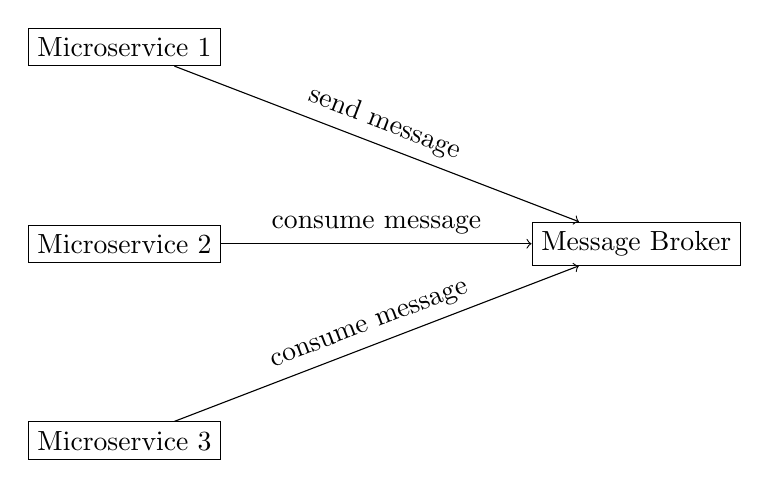
\begin{tikzpicture}[node distance=2.5cm]
  % Define nodes
  \node (microservice1) [rectangle,draw] {Microservice 1};
  \node (microservice2) [rectangle,draw,below of=microservice1] {Microservice 2};
  \node (messagebroker) [rectangle,draw,right of=microservice2,xshift=4cm] {Message Broker};
  \node (microservice3) [rectangle,draw,below of=microservice2] {Microservice 3};

  % Draw edges
  \draw [->] (microservice1) -- node[pos=.5, above, sloped] (TextNode) {send message} (messagebroker);
  \draw [->] (microservice2) -- node[pos=.5, above, sloped] (TextNode) {consume message} (messagebroker);
  \draw [->] (microservice3) -- node[pos=.5, above, sloped] (TextNode) {consume message} (messagebroker);
\end{tikzpicture}
\caption{\textbf{Asynchronous Communication using a message broker.} \\
Microservice 1 sends messages to the message broker. Microservice 2 and 3 consume these messages by contacting the message broker.}
\label{fig:ImageAsyncMBC}
\end{figure}

Contrary to RESTful asynchronous communication, other microservice systems use message-based asynchronous communication.
These systems use messages or events to facilitate communication between its microservices.
These messages or events are typically sent using a messaging system (e.g., Java Message Service, JMS \footnote{https://www.oracle.com/technical-resources/articles/java/intro-java-message-service.html}) or a message broker (e.g., Apache Kafka \footnote{https://github.com/berndruecker/Dowing-retail/tree/master/kafka/java} or RabbitMQ \footnote{https://www.rabbitmq.com}).
After the microservice has sent the message to the message broker, other microservices can consume the messages in the broker.
This communication pattern is depicted in \autoref{fig:ImageAsyncMBC}.
The messaging systems or brokers provide a reliable, scalable and decoupled way for the microservices to communicate with each other.
Using a message broker also allows for better system performance \cite{Singh2021}.


\subsection{Reverse Engineering}
\label{sec:Foundation:SAR}
Reverse engineering is a Software Architecture Extraction (SAR) technique that uses the artifacts of the system (e.g., source code, logs) to analyze the system.
Vital for building the architecture of the software-system is information about the communication between the different components.
This information is extracted using either a static (using only static inputs, e.g. source code), dynamic (using runtime information, e.g. logs) or hybrid (using both) approach.
In the context of asynchronous communication, a static extraction algorithm would in the case of a RESTful asynchronous communication, analyze the HTTP calls made in code to determine the relationships between the components.
In the case of message-based communication, a static approach is unable to extract a useful architecture, since message-based systems exchange those messages only at runtime and thus the required information about which components communicate with each other can only be retrieved as part of a dynamic or hybrid analysis. \cite{Singh2021,Mayer2018}


\subsection{Palladio Component Model}
\label{sec:Foundation:PCM}
%CG
The Palladio Component Model (PCM) is a meta-model for the description of component-based software \cite{Becker2008}.
It is used to predict the performance properties of component-based software at design-time by specifying a model of the system, its components and how the system is going to be used.
A PCM consists of four main views that represent the aspects of the system.
The Component View represents the functional structure of the system, i.e. the components, their interfaces and, the dependencies between them.
The Resource View represents the resources (e.g., CPU, memory, databases, libraries) required by the system.
The Allocation View shows, which components are allocated to which resources.
Finally, the Repository View represents the data structures and operations provided by the system's components as well as the relationships between them. \cite{Becker2008}
